\documentclass{oci}
\usepackage[utf8]{inputenc}
\usepackage{booktabs}
\usepackage{array}
\usepackage{tabularx}
\usepackage{color}


\title{El juego del laberinto}

\renewcommand{\ttdefault}{cmtt}
\newcommand*{\tabbox}[2][t]{\vspace{0pt}\parbox[#1][2.3\baselineskip]{20em}{\strut#2\strut}}
  \newcolumntype{V}{>{\centering\arraybackslash} m{.4\linewidth} }
\def\bgcolor{\par\setbox0\vbox\bgroup}
\def\endbgcolor{\egroup\fboxsep0pt \noindent\colorbox[gray]{0.95}{\usebox0}\par}

\begin{document}
\begin{problemDescription}
  El siguiente problema es un entretenido juego donde debes ayudar a Olonso a cumplir diferentes misiones.
  Nuestro personaje estará atrapado en distintos laberintos y tú debes ayudarlo a recoger algunos objetos para que pueda escapar.
  Para lograrlo solo puedes indicarle un conjunto limitado de acciones para que realice.
  
En el dibujo de más abajo se explica una situación en la que se puede encontrar nuestro personaje.
  Olonso está representado con un triángulo y la punta indica en qué dirección esta mirando.
En este caso Olonso está mirando hacia arriba.
Los objetos que debe recolectar están representados con círculos y solo es necesario pasar por encima de ellos para recogerlos.
En este caso hay un solo objeto.

\begin{center}
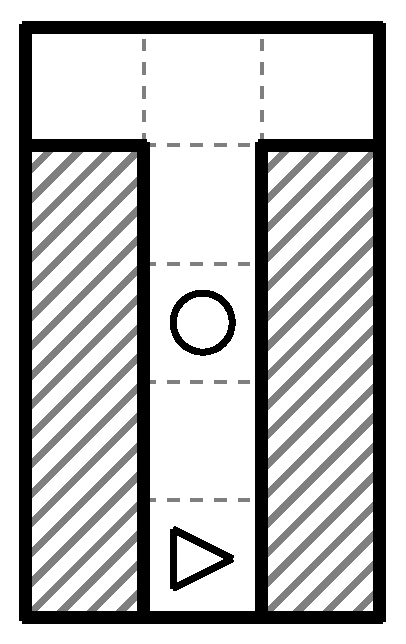
\includegraphics[angle=90,scale=0.5]{laberintos/ejemplo1-1.eps}
\end{center}

\subsection*{Instrucciones básicas}
Las instrucciones básicas que puedes dar a Olonso para que se mueva por el laberinto son las siguientes.
\begin{itemize}
\item \texttt{avanzar} --- Indica a Olonso que debe avanzar una posición hacia la dirección en la que está mirando.
En caso de haber una pared al frente esta instrucción no tiene efecto.
\item \texttt{girar derecha} --- Indica a Olonso que debe girar noventa grados hacia la derecha.
\item \texttt{girar izquierda} --- Indica a Olonso que debe girar noventa grados hacia la izquierda.
\end{itemize}

\subsubsection*{Ejemplo 1}
En el siguiente ejemplo se muestra el comportamiento de nuestro personaje paso a paso dada una secuencia de instrucciones.

\begin{center}
  \begin{tabular}{|V|V|}
    \hline
    \tabbox{\texttt{\# Configuración inicial}}        &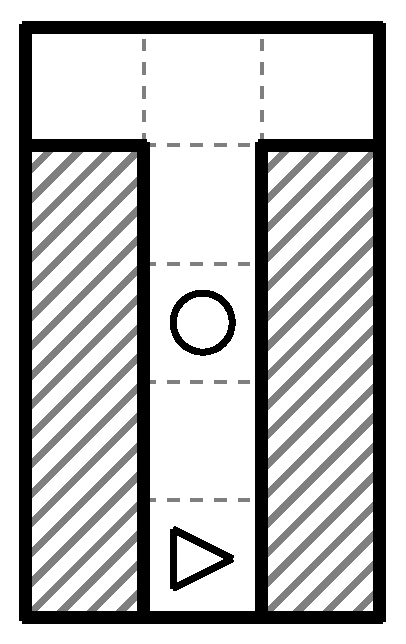
\includegraphics[angle=90, scale=0.25]{laberintos/ejemplo1-1.eps}\\
    \tabbox{\texttt{avanzar \# no tiene efecto}}      &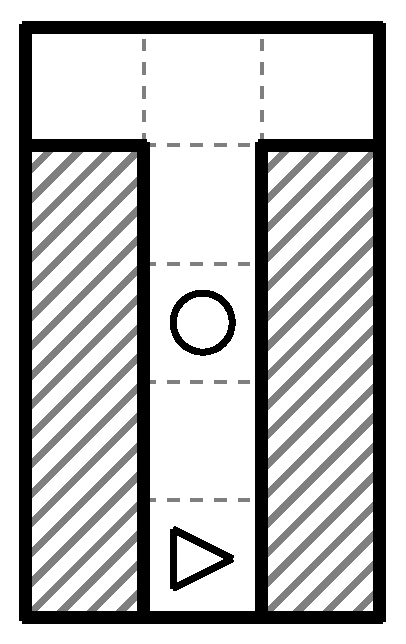
\includegraphics[angle=90, scale=0.25]{laberintos/ejemplo1-1.eps}\\
    \tabbox{\texttt{girar izquierda}}                 &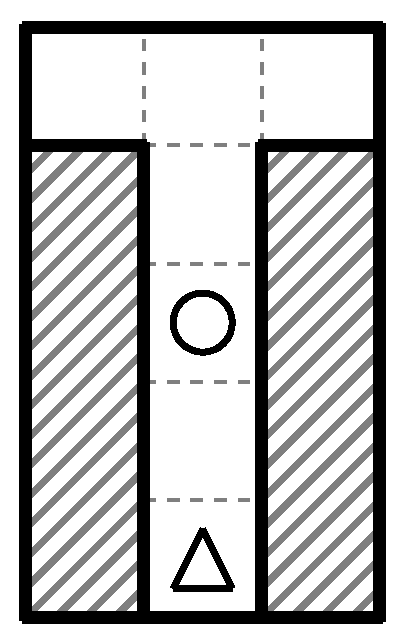
\includegraphics[angle=90, scale=0.25]{laberintos/ejemplo1-2.eps}\\
    \tabbox{\texttt{avanzar}}                         &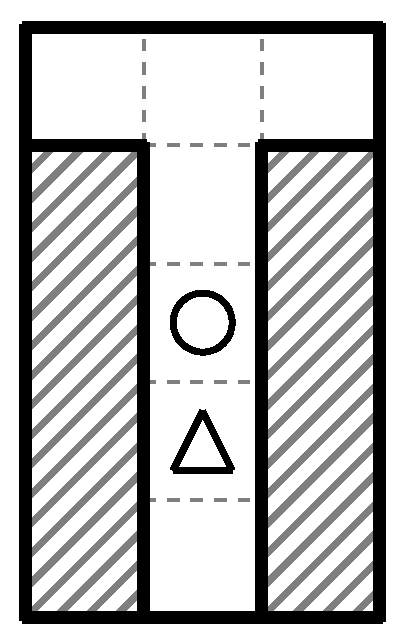
\includegraphics[angle=90, scale=0.25]{laberintos/ejemplo1-3.eps}\\
    \tabbox{\texttt{avanzar \# Recoge el objeto}}     &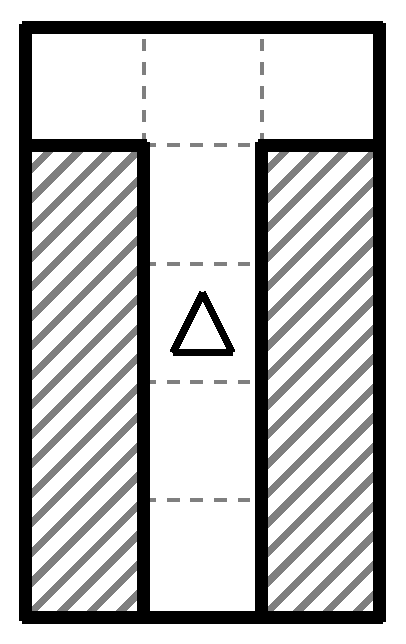
\includegraphics[angle=90, scale=0.25]{laberintos/ejemplo1-4.eps}\\
    \hline
  \end{tabular}
\end{center}



\subsubsection*{Instrucción repetir}
Además de las instrucciones básicas también es posible repetir una secuencia de instrucciones de la siguiente forma.

\begin{verbatim}
repetir:
...
fin repetir;
\end{verbatim}

Esta instrucción ejecutará todas las instrucciones que se encuentran entre los delimitadores \texttt{repetir:} y \texttt{fin repetir;}.
Las instrucciones terminarán de repetirse cuando se hayan recolectado todos los objetos.
La ejecución de instrucciones terminará sin importar si quedaban más acciones por realizar.
Recuerda que para recoger los objetos solo es necesario pasar por sobre de ellos.

\subsubsection*{Ejemplo 2}
A continuación se muestra un escenario y una secuencia de instrucciones que logra recolectar todos los objetos.

\begin{minipage}{0.5\linewidth}
  \centering
  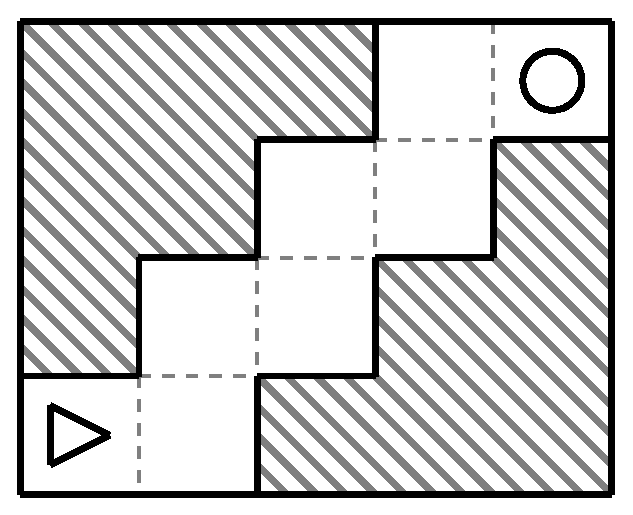
\includegraphics[scale=0.45]{laberintos/ejemplo2.eps}
\end{minipage}
\begin{minipage}{0.5\linewidth}
  \centering
 \bgcolor{}
\begin{verbatim}

  repetir:
    avanzar
    girar izquierda
    avanzar
    girar derecha
  fin repetir;
\end{verbatim}
 \endbgcolor{}
\end{minipage}

Debes tener cuidado con la instrucción \texttt{repetir} pues Olonso podría moverse sin parar en caso de que no recolectar todos los objetos.

\subsubsection*{Instrucción condicional}
Finalmente Olonso también puede tomar decisiones en base a lo que hay a su alrededor.
Para eso posees la siguiente instrucción condicional.

\begin{verbatim}
si [condición]:
...
sino:
...
fin si;
\end{verbatim}
  
Esta instrucción permite decidir que instrucciones realizará Olonso dependiendo de si una condición se cumple o no.
Si la condición que se evalúa es cierta, entonces Olonso realizará las instrucciones que se encuentran entre los delimitadores `\texttt{si [condicon]:}' y `\texttt{sino:}', en caso contrario realizará las instrucciones que se encuentran entre `\texttt{sino:}' y `\texttt{fin si;}'.
Puedes poner lo que desees dentro, incluso más instrucciones condicionales anidadas o ninguna instrucción.

La condición que se evalúa puede ser una de las siguientes:

\begin{itemize}
\item \texttt{hay camino adelante} --- Determina si hay camino hacia adelante.
En otras palabras esta condición será cierta si la instrucción avanzar resultará en que Olonso efectivamente se mueva hacia adelante.
\item \texttt{hay camino izquierda} --- Determina si hay camino hacia la izquierda de Olonso. 
\item \texttt{hay camino derecha} --- Determina si hay camino hacia la derecha de Olonso. 
\end{itemize}

Notar que solo tienes estas condiciones y ninguna más.
En particular no puedes preguntar por la negación de estas.

\subsubsection*{Ejemplo 3}
A continuación se muestra una secuencia de instrucciones que ocupa la instrucción condicional para recolectar todos los objetos del laberinto que se muestra en la imagen.

\begin{minipage}{0.5\linewidth}
  \centering
  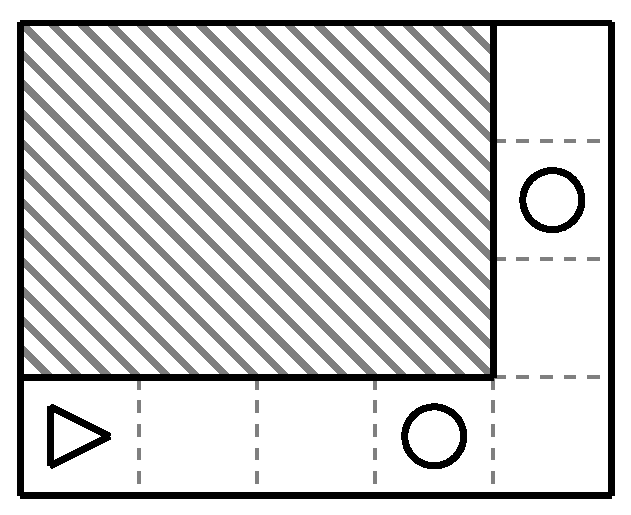
\includegraphics[scale=0.45]{laberintos/ejemplo3.eps}
\end{minipage}
\begin{minipage}{0.5\linewidth}
  \centering
  \bgcolor{}
\begin{verbatim}

  repetir:
    si hay camino izquierda:
      girar izquierda
      avanzar
    sino:
      avanzar
    fin si;
  fin repetir;
\end{verbatim}
  \endbgcolor{}
\end{minipage}

\end{problemDescription}

\section*{Detalles de Implementación}
Para este problema debes enviar {\bf archivos especificando las instrucciones que debe realizar Olonso}.
Cada subtarea describe ciertas condiciones y un laberinto que debe atravesar Olonso.
Para cada subtarea debes enviar un archivo distinto que especifique las instrucciones que debes darle a Olonso para que logre recolectar todos los objetos del laberinto.

Los archivos deben ser en texto plano y contener {\bf una instrucción por línea}.
Las instrucciones son ejecutadas en el orden en que son dadas en el archivo.
Las líneas en blanco y los espacios extras son ignorados, pero debes respetar el nombre exacto de las instrucciones.
El símbolo \verb~#~ indica un comentario; cualquier texto que le sigue, hasta el final de la línea, es ignorado.

No es necesario que envíes todos los archivos cada vez. En caso de no subir uno, se agregará automáticamente el último enviado (si es que existe).
De esta forma te puedes concentrar en una subtarea a la vez.

Al envíar un archivo si haces click en \texttt{details} y luego en alguna subtarea podrás obtener información de tus errores.


\section*{Subtareas y puntaje}

\subsubsection*{Subtarea 1 -- 30 puntos}
\begin{minipage}{0.5\linewidth}
  \centering
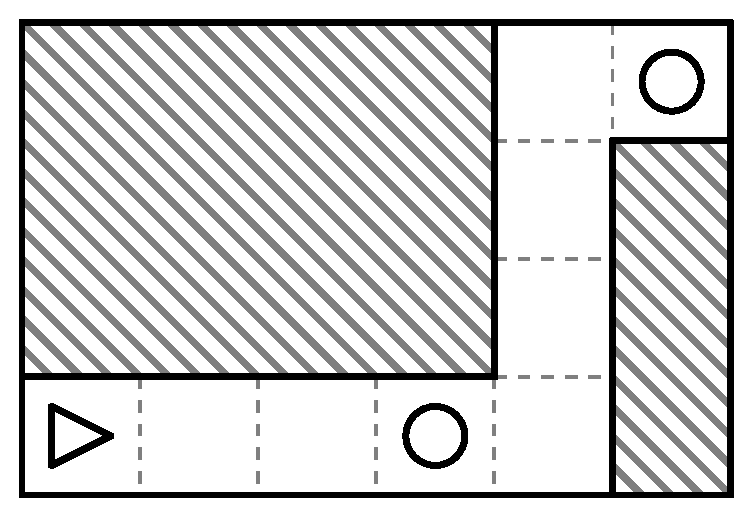
\includegraphics[scale=0.5]{laberintos/Subtarea1.eps}
\end{minipage}
\begin{minipage}{0.45\linewidth}
Para esta subtarea no tienes restricciones, sólo debes recoger todos los objetos.
\end{minipage}

\subsubsection*{Subtarea 2 -- 30 puntos}
\begin{minipage}{0.5\linewidth}
  \centering
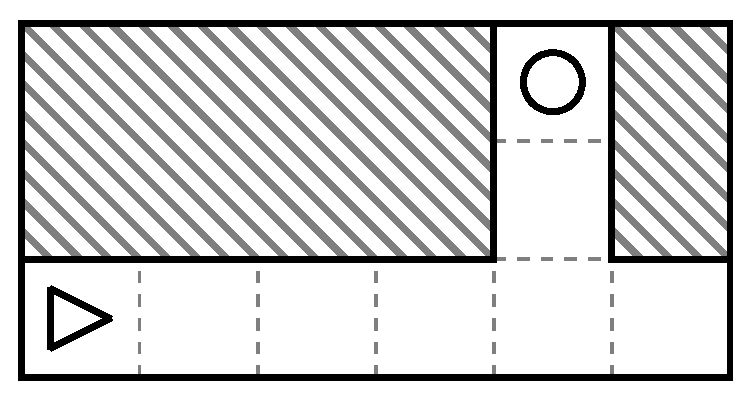
\includegraphics[scale=0.5]{laberintos/Subtarea2.eps}
\end{minipage}
\begin{minipage}{0.45\linewidth}

Este laberinto se puede resolver con las siguientes instrucciones:
\begin{verbatim}
  repetir:
    si hay camino izquierda:
      girar izquierda
      avanzar
    sino:
      avanzar
    fin si;
  fin repetir;
\end{verbatim}

Para esta subtarea debes resolverlo usando \textbf{solo la condición `hay camino adelante'} para las instrucciones condicionales.
Además solo puedes usar la \textbf{instrucción `avanzar' 3 veces}.
\end{minipage}

\subsubsection*{Subtarea 3 -- 40 puntos}
\begin{minipage}{0.5\linewidth}
  \centering
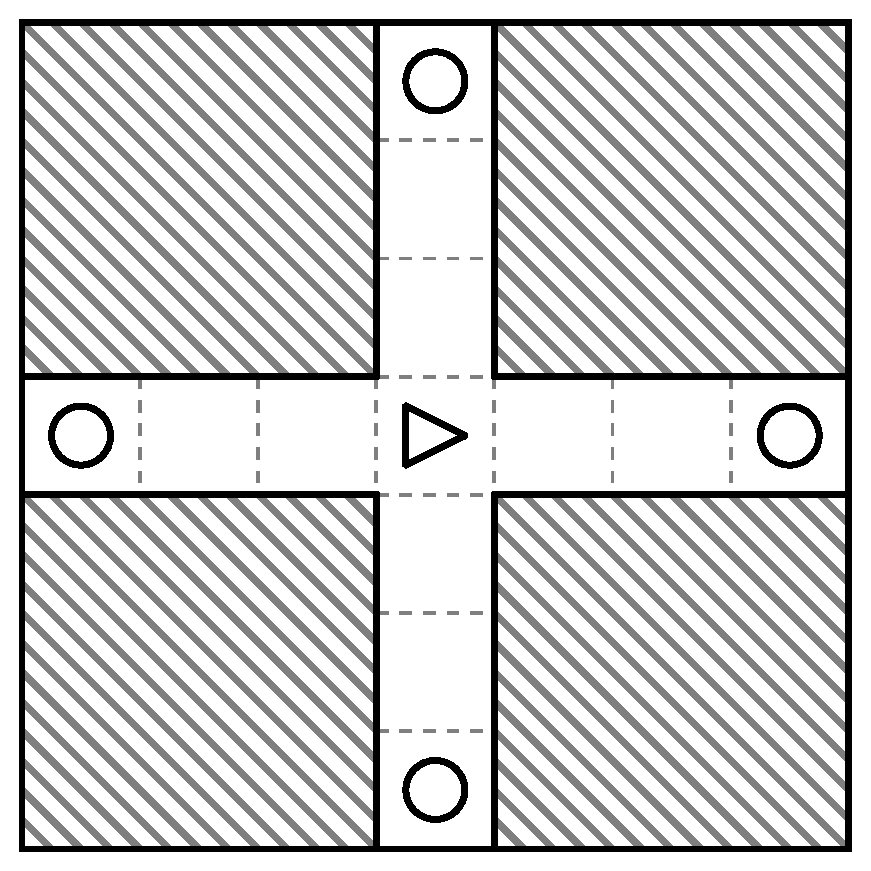
\includegraphics[scale=0.5]{laberintos/Subtarea3.eps}
\end{minipage}
\begin{minipage}{0.45\linewidth}
En esta subtarea debes resolver el laberinto usando \textbf{no más de 10 instrucciones `avanzar'}.
\end{minipage}


% \begin{sampleDescription}
% \sampleIO{sample}
% \sampleIO{sample}
% \end{sampleDescription}

\end{document}
